\chapter{Context}
\section{Use case: TU Delft (working title)}
% Matthijs
% Information about location
This projects main area of interest is the campus of the TU Delft. There are more than 20.000 students using the campus on more than 150 hectares. This emphasises even more the magnitude of this project. The network logs the devices connected to the eduroam access points, which implicitly means logging the (approximate) location of the person carrying the device and more information. This tracking data can be used to derive information about the personality of the person carrying the device, such as the distinction between staff and students, based on the tracked locations. Connection to the Wi-Fi eduroam network is free of charge and requires only a NetID, which all students and staff get upon registration at the university. \\\\
It is very important to understand, that 'no data is also data'. This means that a devices that is not being tracked by any access point for a period of time, is either off-campus or disconnected and still on campus. This provides valuable information when researching the movement patterns. This will be further discussed in the \autoref{preprocessing}. \\\\
The eduroam network of the TU Delft campus consists of 1730 access points, distributed over more than 30 buildings. The data is collected for each of the access points over a period of little more than 3 months. The logs are stored in a database on a virtual server, where it is accessible to the three project groups and the Geomatics staff. The data that is collected and the storage in the database is further described in \autoref{datadescription}. \\\\
The department of Facility Management and Real Estate (FMRE) is the main client for the entire Synthesis Project. They would like to know how the campus is being used, what the hotspots on campus and in buildings are, when people travel the most from one building to another and which buildings are most visited.

\section{Previous research: Rhythm of the campus}
% Matthijs
% Summary of their summary
In the fall of 2014, similar research was conducted during another edition of the Geomatics Synthesis Project. The group "Rhythm of the campus" investigated the use of the Library and the Aula of the TU Delft, to gain insight in patterns the use of the facilities of the Library and Aula. This section will give a short summary of their research (\cite{rhythmofthecampus}).\\\\
During the project, the group used passive Wi-Fi monitoring to detect users of the TU Delft Library and the Aula to gain insight in the occupation, in request of FMRE. They used BlueMark sensors at the Library, Aula and 5 other faculties for a period of one week and collected ground truth data for 2 days. Due to its sheer size, the raw data was difficult to process. The data was filtered from static devices and outliers and the data analysis resulted in identification of the occupation of the Library and the Aula. The end results was a dashboard which visualized the sensor network, data analysis and pattern recognition to help the client in the decision making process.\\\\

This research was different from the research conducted in this Synthesis Project, mainly due the larger size of the eduroam network and the ability to track everybody using the Wi-Fi network.

\section{Privacy}
% Balazs

\section{Data validity and accuracy}
% Balazs

\section{Representativeness}
% Xander

\section{Data description and System of APs}\label{datadescription}
\subsection{Data description}\label{datadescription}
% this is a comment
% normal text
This section will describe the main datasource within the Synthesis Project; a PostgreSQL database containing the logs from the Wi-Fi scanners on the TU Delft campus. Each row in the wifilog table provides a data value for each column (\autoref{segmentwifilog}).


\begin{table}[H]
	\centering
	\captionsetup{justification=centering}
	\caption{A segment of the main datasource; the wifilog table}
	\label{segmentwifilog}
	\begin{tabular}{@{}lllllllll@{}}
		\toprule
		\textbf{username} & \textbf{mac} & \textbf{asstime} & \textbf{}  & \textbf{maploc}                                                     & \textbf{sesdur} & \textbf{snr} & \textbf{ssi} & \textbf{importfile}          \\ \midrule
		j85cCQrGQa..      & l6iOu+xxOq.. & 14-4-2016 12:30  & A-23-0-029 & System Campus \textgreater 23-CITG \textgreater 4e Verdieping       & 1:32:02         & 35           & -57          & 20160414-wifitracking.csv.gz \\
		wrBqMLL+j..       & f2Pw/PMb4/.. & 14-4-2016 7:49   & A-23-0-035 & System Campus \textgreater 23-CITG \textgreater 5e \& 6e Verdieping & 5:32:16         & 37           & -56          & 20160414-wifitracking.csv.gz \\
		wrBqMLL+j..       & f2Pw/PMb4/.. & 14-4-2016 13:22  & A-23-0-035 & System Campus \textgreater 23-CITG \textgreater 5e \& 6e Verdieping & 0:40:20         & 46           & -50          & 20160414-wifitracking.csv.gz \\
		wrBqMLL+j..       & f2Pw/PMb4/.. & 14-4-2016 14:02  & A-23-0-093 & System Campus \textgreater 23-CITG \textgreater 5e \& 6e Verdieping & 1:27:13         & 11           & -86          & 20160414-wifitracking.csv.gz \\
		wrBqMLL+j..       & f2Pw/PMb4/.. & 14-4-2016 15:29  & A-23-0-091 & System Campus \textgreater 23-CITG \textgreater 5e \& 6e Verdieping & 0:05:08         & 30           & -65          & 20160414-wifitracking.csv.gz \\
		wrBqMLL+j..       & f2Pw/PMb4/.. & 14-4-2016 15:34  & A-23-0-035 & System Campus \textgreater 23-CITG \textgreater 5e \& 6e Verdieping & 1:42:32         & 29           & -65          & 20160414-wifitracking.csv.gz \\
		J0IwA+vpcS..      & HkLY1UMpBV.. & 14-4-2016 11:33  & A-23-0-035 & System Campus \textgreater 23-CITG \textgreater 5e \& 6e Verdieping & 1:27:40         & 33           & -59          & 20160414-wifitracking.csv.gz \\
		J0IwA+vpcS..      & HkLY1UMpBV.. & 14-4-2016 13:01  & A-23-0-035 & System Campus \textgreater 23-CITG \textgreater 5e \& 6e Verdieping & 1:01:01         & 26           & -68          & 20160414-wifitracking.csv.gz \\
		J0IwA+vpcS..      & HkLY1UMpBV.. & 14-4-2016 14:02  & A-23-0-035 & System Campus \textgreater 23-CITG \textgreater 5e \& 6e Verdieping & 3:30:19         & 25           & -68          & 20160414-wifitracking.csv.gz \\
		J0IwA+vpcS..      & HkLY1UMpBV.. & 14-4-2016 17:32  & A-23-0-035 & System Campus \textgreater 23-CITG \textgreater 5e \& 6e Verdieping & 0:40:05         & 27           & -69          & 20160414-wifitracking.csv.gz \\ \bottomrule
	\end{tabular}
\end{table}

The data value for each attribute (column) in the wifilog table will be described in more detail. 
\\\\
\textbf{username:}\\
The username column provides the username, as a hashed text. Every user has a unique username, but can appear in the data more than once.
\\\\
\textbf{mac:}\\
The mac column provides the media access control adress (MAC address), as a hashed text. The MAC address is a unique identifier assigned to a specific piece of hardware, such as the network adapter located in Wi-Fi devices (mobile phones, tablets, laptops etc.). So, it would be possible that a user can have more than one device connected to the Wi-Fi eduroam network.
\\\\
\textbf{asstime:}\\
The asstime is the time of which a connected device is recorded by the system.
\\\\
\textbf{apname:}\\
The apname is the name assigned to the access point. Every access point has a unique name. 
\\\\
\textbf{maploc:}\\
The maploc describes the location of the access point. There could be multiple access points with the same maploc. For instance, there are 31 access points located on the ground floor of the Faculty of Architecture.
\\\\
\textbf{sesdur:}\\
The sesdur describes the session duration of which a device is connected to the access point. Because this is not as straightforward as it seems, this will be explained more extensively.
\\\\
bladibla figure shows the the frequency of session durations.
\\\\
picture
\\\\
The figure shows a large peak at exactly 5 minutes, a peak at approximately 5 minutes and decreasing peaks after a time interval of approximately 5 minutes. It looks like it is recording in a certain time interval in which the device is (still) connected. \\\\
In order to justify this, the query below is used to see the asstimes (and time to next asstime)
\begin{lstlisting}[language=SQL]
select *, asstime_next-asstime as difference
from (
	select count(*),asstime, lead(asstime) over (order by asstime) asstime_next
	from wifilog
	where extract(day from asstime) = 4
	and extract(month from asstime) = 4
	and extract(year from asstime) = 2016
	group by asstime
	order by asstime) as subquery
\end{lstlisting}


\begin{table}[H]
	\centering
	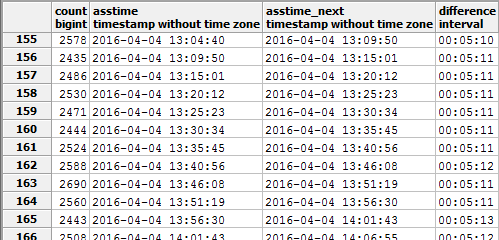
\includegraphics[scale=1]{timetonextscan.PNG}
 tiofigure:n{The time and time to next scan at a random day}
	\label{timetonextscan}
	\begin{tabular}{@{}llll@{}}
		\toprule
		count & asstime        & asstime\_next  & difference \\ \midrule
		2578  & 4-4-2016 13:04 & 4-4-2016 13:09 & 0:05:10    \\
		2435  & 4-4-2016 13:09 & 4-4-2016 13:15 & 0:05:11    \\
		2486  & 4-4-2016 13:15 & 4-4-2016 13:20 & 0:05:11    \\
		2530  & 4-4-2016 13:20 & 4-4-2016 13:25 & 0:05:11    \\
		2471  & 4-4-2016 13:25 & 4-4-2016 13:30 & 0:05:11    \\
		2444  & 4-4-2016 13:30 & 4-4-2016 13:35 & 0:05:11    \\
		2524  & 4-4-2016 13:35 & 4-4-2016 13:40 & 0:05:11    \\
		2588  & 4-4-2016 13:40 & 4-4-2016 13:46 & 0:05:12    \\
		2690  & 4-4-2016 13:46 & 4-4-2016 13:51 & 0:05:11    \\
		2560  & 4-4-2016 13:51 & 4-4-2016 13:56 & 0:05:11    \\ \bottomrule
	\end{tabular}
\end{table}

         
\autoref{timetonextscan} shows that the time to the next scan is 5 minutes and several seconds in all cases. Most important is to know that all access points are recording the connected device(s) is at the same time. 
\\\\                                                        
\autoref{sesdur_example} will be used to explain the way the time interval of approximately 5 minutes is coming back in the session duration.
                                                                       
% Please add the following required packages to your document preamble:
% \usepackage{booktabs}
\begin{table}[]
	\centering
	\captionsetup{justification=centering}
	\caption{Varying session durations}
	\label{sesdur_example}
	\begin{tabular}{@{}lllllll@{}}
		\toprule
		\textbf{id} & \textbf{username} & \textbf{mac} & \textbf{asstime} & \textbf{apname} & \textbf{maploc}                                                                     & \textbf{sesdur} \\ \midrule
		1           & oHh0SzXKc0..      & WWW0Cdd++v.. & 1-4-2016 10:13   & A-12-0-104      & System Campus \textgreater 12-Kramerslab \& Proeffabriek \textgreater !e Verdieping & 0:05:00         \\
		2           & oHh0SzXKc0..      & WWW0Cdd++v.. & 1-4-2016 10:18   & A-132-0-064     & System Campus \textgreater 32-OCP-IO \textgreater 1e Verdieping                     & 0:20:27         \\
		3           & oHh0SzXKc0..      & WWW0Cdd++v.. & 1-4-2016 11:36   & A-132-0-105     & Root Area                                                                           & 0:15:22         \\
		4           & oHh0SzXKc0..      & WWW0Cdd++v.. & 1-4-2016 11:51   & A-132-0-066     & System Campus \textgreater 32-OCP-IO \textgreater 1e Verdieping                     & 0:20:35         \\
		5           & oHh0SzXKc0..      & WWW0Cdd++v.. & 1-4-2016 14:01   & A-132-0-069     & System Campus \textgreater 32-OCP-IO \textgreater 1e Verdieping                     & 0:05:43         \\
		6           & oHh0SzXKc0..      & WWW0Cdd++v.. & 1-4-2016 14:06   & A-132-0-133     & System Campus \textgreater 32-OCP-IO \textgreater 4e Verdieping                     & 0:05:18         \\
		7           & oHh0SzXKc0..      & WWW0Cdd++v.. & 1-4-2016 14:12   & A-132-0-066     & System Campus \textgreater 32-OCP-IO \textgreater 1e Verdieping                     & 0:05:10         \\
		8           & oHh0SzXKc0..      & WWW0Cdd++v.. & 1-4-2016 14:17   & A-132-0-104     & System Campus \textgreater 32-OCP-IO \textgreater 2e Verdieping                     & 0:05:10         \\
		9           & oHh0SzXKc0..      & WWW0Cdd++v.. & 1-4-2016 14:22   & A-132-0-067     & System Campus \textgreater 32-OCP-IO \textgreater 1e Verdieping                     & 0:05:10         \\
		10          & oHh0SzXKc0..      & WWW0Cdd++v.. & 1-4-2016 14:27   & A-132-0-066     & System Campus \textgreater 32-OCP-IO \textgreater 1e Verdieping                     & 0:10:21         \\ \bottomrule
	\end{tabular}
\end{table}
                                                                                                                                                                                                                                                                                                                                                                                                                                                                                                                                                                                                                                                                                                                                                                                                                                                   
The first record shows the device is not connected to any of the access points on the campus in the subsequent moment of recording, resulting in a session duration of exactly 5 minutes. In the last record in \autoref{sesdur_example} shows the result of a device that is still connected to the same access point at the subsequent moment of recording. In this case the session duration will be 10 minutes and 21 seconds. This is the time interval between the first moment the device is recorded and the first time the device is not recorded by the same access point anymore. The record with id number 6 describes a situation in which the device is connected to an access point at the moment of recording and connected to another access point at the subsequent moment of recording, the session duration is 5 minutes and 18 seconds in this case. This is the time interval between the two moments of recording.\\\\

\textbf{snr:}
The signal to noise (snr) describes a measurement that compares the signal strength to the level of background noise (in dB).\\\\
\textbf{rssi:} \\
The received signal strength indicator (rssi) describes the received signal strength (in dB).

\subsection{System of APs}\label{systemofaps}
This section will describe the current layout of access points (APs) on the TU Delft campus. The exact location of APs in a building is not known, but for the Faculty of Architecture. Therefore the system of APs in the Faculty of Architecure will be described in more detail. 
\\
The total number of access points, distributed over more than 30 buildings. 
Mostly placed on walls or ceilings. Every access point has a floor location, but this does not mean only people on that floor can connect to that access point. Also rooms with high ceilings, such as the orange hall in bk, can have access point located at first floor level but also serve people 

